\documentclass[a4paper,12pt]{scrreprt}
    %% Used for changing geometry of the page
    %% Cover page text cannot overlay cover sketching/style 
    %% https://ctan.org/pkg/geometry?lang=en
\usepackage{geometry}
    %% Changes language of some packages protocols
    %% e.g., when captioning images: Figure 1. -> Figura 1.
    %% https://ctan.org/pkg/babel?lang=en
\usepackage[portuguese]{babel}
    %% Used for special fonts
    %% Cannot be compiled with pdflatex
    %% https://ctan.org/pkg/fontspec?lang=en
\usepackage{fontspec}
    %% Arial FONT
    \setmainfont{Arial}

    %% More colors and color options
    %% https://ctan.org/pkg/xcolor?lang=en
    %% https://ctan.org/pkg/colortbl?lang=en
\usepackage{xcolor,colortbl}
    %% More tabular options, like dashed/dotted lines
    %% https://ctan.org/pkg/arydshln?lang=en
\usepackage{arydshln}
    %% List of acronyms
    %% https://ctan.org/pkg/nomencl?lang=en
\usepackage[intoc]{nomencl}
    %% Must be called to init nomencl environment  
    \makenomenclature
    %% More images options/settings
    %% https://ctan.org/pkg/graphicx?lang=en
\usepackage{graphics}
    %% Defining subdirectories to image path enviornment
    %% \graphicspath{{sub1}{sub2}...{subN}}
    \graphicspath{{images}}
    
    %% used to handle cross-referencing commands in LaTeX to produce hypertext links in the document
    %% https://ctan.org/pkg/hyperref?lang=en
\usepackage{hyperref}
    %% math environments
    %% https://ctan.org/pkg/amsmath?lang=en

    %% settings
    \hypersetup{
        colorlinks,
        citecolor=black,
        filecolor=black,
        linkcolor=black,
        urlcolor=black
    }

\usepackage{amsmath}
    %% Defining backgrouns, used to make the cover
    %% https://ctan.org/pkg/background?lang=en
\usepackage[some]{background}
    %% Used to make drawings or complex graphics
    %% http://pgf.sourceforge.net/pgf_CVS.pdf
\usepackage{tikz}
    %% Tikz library to point operations ((x1,y1) + (x2,y2))
    \usetikzlibrary{calc}

%% Defining sfdefault font and default font for document
\renewcommand{\familydefault}{\sfdefault}


%% Costume made cover 
%% From there you can use \makecover command to build the cover


%==========================================================================
% DOCUMENT
%==========================================================================

\begin{document}
%% Blue cover color
\definecolor{titlepagecolor}{RGB}{49,132,155}

%==========================================================================
% COLORED BAR ON THE LEFT SIDE
%==========================================================================

\backgroundsetup{
    scale=1, 
    angle=0, 
    opacity=1,
    contents={
        \begin{tikzpicture}[remember picture,overlay]
            \path [fill=titlepagecolor] 
                (current page.north west) -- ($(current page.north west) + (5,0)$)
                -- ($(current page.south west) + (5,0)$)-- (current page.south west); 
            \node[color=white] at ($(current page.south west) + (2.5,4)$) {\bfseries {\fontsize{120}{60} \textsf{ B}}};
            \node[color=titlepagecolor] at ($(current page.south west) + (5.8,4)$) {\bfseries {\fontsize{120}{60} \textsf{ D}}};
        \end{tikzpicture}
    }
}

%==========================================================================
% TITLE PAGE INFO
%==========================================================================

%% Changes values in this field to show information in the cover and back cover about your team/project


%% TITLE
\title{Mademoiselle Borges: Um Sistema de Bases de Dados para a Gestão de Eventos em Eventopolis}

%% AUTHORS
\author{
    Bruno Gi\~ao (A96544) %%% Bruno Dias da Gião
  \qquad
    Jo\~ao Pereira (A95375) %%% João Luís da Cruz Pereira
  \qquad
    Helena Salazar (A75635) %%% Maria Helena Alves Machado Marques Salazar
  \qquad
    Tiago Teixeira (A97666) %%% Tiago Emanuel Lemos Teixeira
}
%% Date

\date{Novembro, 2023}

%% Course
\newcommand{\Course}{Licenciatura em Ciências da Computação}

%% Department
%%% \newcommand{\Department}{Escola de Engenharia}

%% UniName
\newcommand{\UniName}{Universidade do Minho}

%% UniPic
\newcommand{\UniPic}{
\includegraphics[scale=0.09]{images/uminho.png}}

%% University 
\newcommand{\University}{
    \begin{flushleft}
        \UniPic
    \end{flushleft}
    \textcolor{gray}{\small\textbf{\textsf{\UniName}}}\par
    %%% \textcolor{gray!80!white}{\small{\textsf{\Department}}}\par
    \textcolor{gray!70!white}{\small{\textsf{\Course}}}
}

%% UC
\newcommand{\UC}{
    \begin{flushleft}
        \par\textcolor{titlepagecolor}{  \LARGE\textbf{\textsf{Unidade Curricular de \\ Bases de Dados}}}
    \end{flushleft}
}

%% School Year
\newcommand{\SchoolYear}{
    \small{\textsf{Ano Letivo de 2023/2024}}}


%% Define new command to show title, author and date
\makeatletter
\let\Title\@title
\let\Author\@author
\let\Date\@date
\makeatother

%==========================================================================
% CLASSIFICATION SECTION 
%==========================================================================

%% School Year
\newcommand{\ReceptionDate}{}
%% Responsible
\newcommand{\Responsible}{}
%% Evaluation
\newcommand{\Evaluation}{}
%% Observations
\newcommand{\Observations}{}





%% MAKETEMPLATE
\newcommand{\makecover}{

%==========================================================================
% BEGIN COVER PAGE 
%==========================================================================

%% Removes page number on footer
\thispagestyle{empty}

%% No indentation 
\setlength{\parindent}{0em}

%% Put Background defined on \backgroundsetup, in this page
\BgThispage

%% Changing geometry to prevent overlay with text
%% At the end of back cover, geometry is default with \restoregeometry
\newgeometry{top=5cm,left=6cm,right=3cm,bottom=2cm}

%% builds university info defined previously
\University
\vspace{1cm}
%% builds curricular unity info defined previously
\UC
%% builds school year info defined previously
\SchoolYear

\vspace*{4cm}
%% bigger space (i think its the default one) between paragraphs 
\setlength{\parskip}{1em}

%% builds title info defined previously
\par\textbf{\textsf{\huge\Title}}
\vspace{1cm}
%% builds author(s) info defined previously
\par\Author

\vspace{0.5cm}

%% builds date info defined previously
\par\Date
\restoregeometry
\pagebreak

%==========================================================================
% END COVER PAGE 
%==========================================================================

%==========================================================================
% BEGIN BACK COVER PAGE 
%==========================================================================

%% Removes page number on footer
\thispagestyle{empty}

% Changing look of lines in tabular environment 
% Dashed -> dotted 
%% length of dashes
\setlength\dashlinedash{0.3pt}
%% space between dashes
\setlength\dashlinegap{1.5pt}
%% width of dashes
\setlength\arrayrulewidth{1.1pt}


%% This values can be changed in the preamble
\begin{flushright}
\begin{tabular}{ :p{4cm}:p{4cm}: } 
\hdashline
Data de Recepção & \ReceptionDate \\ [2ex]
\hdashline
Responsável & \Responsible \\ [2ex]
\hdashline
Avaliação & \Evaluation \\ [2ex]
\hdashline
Observações & \Observations \\ [7ex]
\hdashline
\end{tabular}
\end{flushright}


\vspace{9cm}
\begin{flushleft}

%% builds title info defined previously
\par\textbf{\textsf{\huge\Title}}
\vspace{1cm}
%% builds author info defined previously
\par\Author

\vspace{0.5cm}

%% builds date info defined previously
\par\Date
\end{flushleft}

\pagebreak
%==========================================================================
% END BACK COVER PAGE 
%==========================================================================
}

\pagenumbering{gobble}

% builds the cover
\makecover

%% smaller footer and header size
\newgeometry{top=3cm,left=3cm,right=3cm,bottom=4cm}

%==========================================================================
% BEGIN OPCIONAL DEDICATÓRIA
%==========================================================================

%%\clearpage
%%\begin{center}
 %%   \thispagestyle{empty}
  %%  \vspace*{\fill}
    
  %%  $<<$/opcional Dedicatória$>>$
    
 %%   \vspace*{\fill}
%%\end{center}
%%\clearpage

%==========================================================================
% END OPCIONAL DEDICATÓRIA
%==========================================================================


%==========================================================================
% BEGIN ABSTRACT PAGE
%==========================================================================



%% Abstract name: \Large font size, flushed left and paragraph skip before abstract content
\renewenvironment{abstract}
 {\par\noindent\textbf{\Large\abstractname}\par\bigskip}
 {}

\begin{flushleft}
\begin{abstract}
    Neste trabalho, foi inicializado o processo do desenho de um Sistema de Bases de Dados na forma da
    contextualiza\c{c}\~ao do problema, visando criar uma \textit{blueprint} s\'olida e demonstrar que, efetivamente,
    \'e justificada a cria\c{c}\~ao do presente Sistema de Bases de Dados,
    o levantamento de requisitos de manipulação, descrição, e controlo e a conceptualização do
    problema com recurso a um diagrama conceptual (\textit{Entity-Relationship Diagram}).
    \par \textbf{\'Area de Aplicação}: Desenho e arquitectura de Sistemas de Bases de Dados.
    \par \textbf{Palavras-Chave}: Bases de Dados Relacionais, Defini\c{c}\~ao de Sistema, SQL, Diagrama Conceptual,
    Recolha de Requisitos.
\end{abstract}
\end{flushleft}


\pagebreak

%==========================================================================
% END ABSTRACT PAGE 
%==========================================================================

%==========================================================================
% BEGIN INDEXES PAGES
%==========================================================================

%% Changes table of content name
%% Portuguese babel default : "Conteúdo"
%% Personally I prefer "índice"
\renewcommand{\contentsname}{Índice}

\tableofcontents

\pagebreak

\listoffigures

\pagebreak

\listoftables

\pagebreak

%==========================================================================
% END INDEXES PAGES 
%==========================================================================


%==========================================================================
% BEGIN INTRODUCTION
%==========================================================================

%% Starting page numbering here
\pagenumbering{arabic}

\chapter{Introdução}
    <<Este primeiro capítulo deverá ter obrigatoriamente as subsecções abaixo apresentadas.>>
    \section{Contextualização}
        <<Nesta secção deverá ser apresentado o contexto no qual se desenvolve o caso de estudo seleccionado.>>
    \section{Apresentação do Caso de Estudo}
        <<Esta secção acolherá uma descrição concisa do caso de estudo seleccionado.>>
    \section{Motivação e Objectivos}
        <<Esta secção acolherá os diversos motivos, acompanhados por uma breve descrição, que conduziram à proposta e ao desenvolvimento do trabalho, assim como a apresentação detalhada dos diversos objectivos a alcançar com a sua realização.>>
    \section{Estrutura do Relatório}
        <<Após a leitura da introdução de um relatório é "simpático" apresentar uma breve descrição daquilo que se vai encontrar nos demais capítulos do relatório.>>

%==========================================================================
% END INTRODUCTION
%==========================================================================


%==========================================================================
% BEGIN SUGESTÕES PARA ESCRITA DO RELATÓRIO
%==========================================================================

\chapter{Sugestões para Escrita do Relatório}

    \section{Sugestões Gerais}
        <<O presente documento deverá servir de base para a escrita do relatório do trabalho realizado.>>\\

        <<O tipo de letra a utilizar deverá ser Arial.. Porém recomenda-se em situações de escrita de excertos de programas a utilização do tipo de letra Courier New.>>\\

        << Alguns estilos documento: Heading1, Heading2, Heading3, Normal e Footnote Text; foram especialmente modificados para os relatórios da presente disciplina.>>\\

        <<Os formatos e estilos de letra não devem estar constantemente a ser modificados ao longo do relatório. Tal situação dará origem a um relatório com um formato e apresentação muito heterogénea e com um aspecto pouco consistente.>>
    \section{Termos Estrangeiros}
        <<Os termos estrangeiros utilizados deverão ser apresentados num formato diferente do resto do texto, por exemplo: Data Warehouse (em itálico) ou "Data Warehouses" (entre aspas), devendo ser evitados sempre que se conheça uma tradução correcta para português. Para validação desses termos existem vários dicionários no mercado que poderão ser úteis.>>
    \section{Tabelas e Figuras}
        <<Caso seja necessário introduzir figuras ou tabelas no corpo do documento, estas devem seguir os formatos que se apresentam de seguida. Qualquer figura ou tabela deverá ter uma legenda associada, devendo esta estar correctamente apresentada no índice respectivo no início do relatório.>>
        

         \begin{figure}[!h]
            \centering
            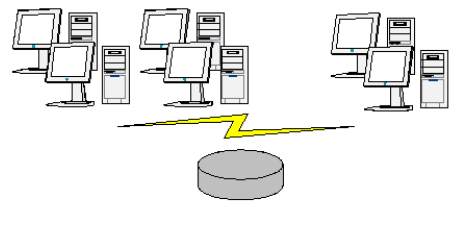
\includegraphics[scale=0.7]{images/example.png}
            \caption{Ilustração de inserção de uma figura e legenda.}
         \end{figure}
        
        \vspace*{0.2cm}
        
        \begin{table}[!h]
            \centering
            \begin{tabular}{|p{2cm}|p{2cm}|p{2cm}|p{2cm}|p{2cm}|}
               \hline
               \rowcolor{gray!20!white}
                Coluna1 & Coluna2 & Coluna3 & & ColunaN \\
                \hline
                        &         &         & &         \\
                \hline
                        &         &         & &         \\
                \hline
                        &         &         & &         \\
                \hline
                        &         &         & &         \\
                \hline
                        &         &         & &         \\
                \hline
            \end{tabular}
            \caption{Ilustração de inserção de uma tabela e sua legenda.}
        \end{table}
        
        
    \section{Siglas e Acrónimos}
        <<A utilização de siglas ou acrónimos deverão, tal como os termos estrangeiros, ser feita com base no seguinte formato: Bases de Dados (BD). Todas as siglas e acrónimos deverão ser apresentadas numa secção própria, no início (a seguir aos índices) ou no final (a seguir ao capítulo das conclusões e trabalho futuro) do relatório.
    \section{Referências Bibliográficas}
        <<A forma de apresentação das referências bibliográficas deverão estar de acordo com as regras definidas pela IEEE. Consultar www.ieee.org>>
    \section{Tipo de Ficheiro}
        <<O relatório poderá ser enviado para o regente da disciplina por correio electrónico num dos seguintes formatos: html, word ou pdf>>
   
        
%==========================================================================
% END SUGESTÕES PARA ESCRITA DO RELATÓRIO
%==========================================================================

%==========================================================================
% BEGIN CONCLUSÕES DE TRABALHO FUTURO
%==========================================================================

\chapter{Conclusões e Trabalho Futuro}
    <<Elaborar uma apreciação crítica sobre o trabalho realizado, apontando os seus pontos fortes e fracos. Adicionalmente, caso se aplique, enunciar eventuais tarefas a realizar futuramente ou novas opções para estender o trabalho realizado.>>


%==========================================================================
% END CONCLUSÕES DE TRABALHO FUTURO
%==========================================================================

%==========================================================================
% BEGIN REFERÊNCIAS
%==========================================================================

%% Changes biblibography name
%% Portuguese babel default : "Bibliografia"
%% Personally I prefer "Referências"
\renewcommand\bibname{Referências}

%% https://www.overleaf.com/learn/latex/bibliography_management_with_bibtex
\begin{thebibliography}{9}
<<Apresentar a lista de referências bibliográficas referidas ao longo do relatório; recomenda-se a utilização do formato Harvard - http://libweb.anglia.ac.uk/referencing/harvard.htm>>
\end{thebibliography}


%==========================================================================
% END REFERÊNCIAS
%==========================================================================

%==========================================================================
% BEGIN LISTA DE SIGLAS E ACRÓNIMOS
%==========================================================================

%% Portuguese babel does not translate this environment
\renewcommand{\nomname}{Lista de Siglas e Acrónimos}

%% Text that can be shown before acronyms list
\renewcommand{\nompreamble}{<<Apresentar uma lista com todas as siglas e acrónimos utilizados durante a realização do trabalho. O formato base para esta lista deverá ser da forma como abaixo se apresenta.>>}

%% acronyms
\nomenclature[01]{\textbf{BD}}{Base de Dados}
\nomenclature[02]{DW}{Data Warehouse}
\nomenclature[03]{OLTP}{On-Line Analytical Processing}
\nomenclature[04]{...}{...}

%% Show acronyms
\printnomenclature



%==========================================================================
% END LISTA DE SIGLAS E ACRÓNIMOS
%==========================================================================


%==========================================================================
% BEGIN ANEXOS
%==========================================================================

%% Why \addchap, instead of \chapter? 
%% \addchap has no numbering but appears in table of contents.
\addchap{Anexos}

    <<Os anexos deverão ser utilizados para a inclusão de informação adicional necessária para uma melhor compreensão do relatório o para complementar tópicos, secções ou assuntos abordados. Os anexos criados deverão ser numerados e possuir uma designação. Estes dados permitirão complementar o Índice geral do relatório relativamente à enumeração e apresentação dos diversos anexos.>>
    
    %% section version of \addchap
    \addsec{Anexo 1}


%==========================================================================
% END ANEXOS
%==========================================================================
\end{document}
